% Figure 1 — Running example threaded through the paper.
% Corporate-email setting. Alice (u) and Bob (v) have never emailed
% (CN=0). Two convex 2-hop cohesive bridges connect them: an upper
% high-cohesion bridge Carol--Dan and a lower bridge Eve--Grace.
% Per Def 6, bridge_c sums core numbers over BOB's neighbours in
% N_2(Alice), i.e. c(Dan) + c(Grace).
%
% Hand-drawn-feel: asymmetric vertical offsets between the two
% bridges, asymmetric horizontal spans, every edge audited.
% Labels are placed OUTSIDE the figure perimeter so they never
% overlap any edge.
%
% EDGE AUDIT (every edge below):
%   Alice--Carol   solid  gray   real 1-hop edge
%   Alice--Eve     solid  gray   real 1-hop edge
%   Alice--Hank    solid  gray   real 1-hop edge (degree asymmetry)
%   Bob--Dan       solid  gray   real 1-hop edge
%   Bob--Grace     solid  gray   real 1-hop edge
%   Carol--Dan     solid  ORANGE real edge, highlighted as upper 2-hop bridge
%   Eve--Grace     solid  ORANGE real edge, highlighted as lower 2-hop bridge
%   Alice--Bob     DASHED gray   candidate future edge (does not yet exist)
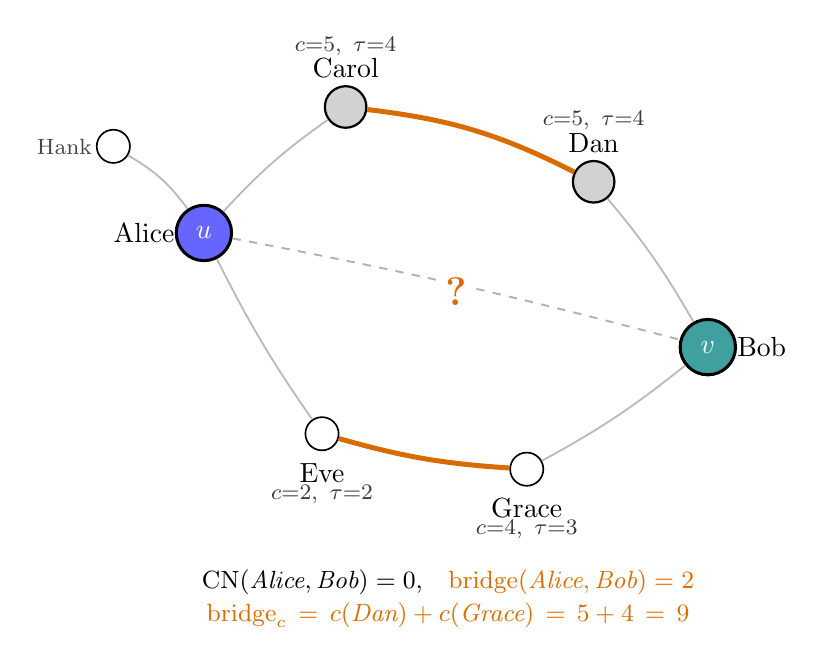
\begin{tikzpicture}[
  every node/.style={font=\rmfamily\normalsize},
  nd/.style={circle,draw,minimum size=12pt,inner sep=0pt,fill=white,
             line width=0.6pt},
  hi/.style={circle,draw,minimum size=15pt,inner sep=0pt,fill=gray!35,
             line width=0.8pt},
  qry/.style={circle,draw,minimum size=20pt,inner sep=0pt,
              line width=1.1pt},
  brg/.style={orange!85!black,line width=1.8pt},
  ed/.style ={gray!55,line width=0.65pt},
  cq/.style ={font=\rmfamily\footnotesize,gray!45!black},
  x=1cm,y=1cm]

  % --- Query nodes: Alice high-left, Bob low-right; intentional tilt
  \node[qry,fill=blue!60,text=white] (u) at (-0.40, 1.85) {$u$};
    \node[anchor=east] at (-0.65, 1.85) {Alice};
  \node[qry,fill=teal!75,text=white] (v) at ( 6.00, 0.40) {$v$};
    \node[anchor=west] at ( 6.25, 0.40) {Bob};

  % --- UPPER bridge nodes (high cohesion). Carol and Dan are NOT at the same y
  \node[hi] (carol) at (1.40, 3.45) {};
    \node[anchor=south] at (1.40, 3.70) {Carol};
    \node[cq,anchor=south] at (1.40, 3.98) {$c{=}5,\ \tau{=}4$};
  \node[hi] (dan)   at (4.55, 2.50) {};
    \node[anchor=south] at (4.55, 2.75) {Dan};
    \node[cq,anchor=south] at (4.55, 3.03) {$c{=}5,\ \tau{=}4$};

  % --- LOWER bridge nodes. Lower bridge is INTENTIONALLY shorter in x-span
  %     and shifted left, so the figure is not a y-mirror.
  \node[nd] (eve)   at (1.10,-0.70) {};
    \node[anchor=north] at (1.10,-0.95) {Eve};
    \node[cq,anchor=north] at (1.10,-1.23) {$c{=}2,\ \tau{=}2$};
  \node[nd] (grace) at (3.70,-1.15) {};
    \node[anchor=north] at (3.70,-1.40) {Grace};
    \node[cq,anchor=north] at (3.70,-1.68) {$c{=}4,\ \tau{=}3$};

  % --- Alice's extra non-bridge contact. We name him "Hank" so the small
  %     circle isn't a stray dot; he's an Alice-only contact who plays no
  %     role in the (Alice, Bob) bridge story.
  \node[nd] (hank) at (-1.55, 2.95) {};
    \node[font=\rmfamily\footnotesize,gray!55!black,anchor=east] at (-1.70, 2.95) {Hank};

  % --- EDGES (audited above) ---
  % Alice's 1-hop edges (real, solid gray)
  \draw[ed] (u) to[bend left=6]   (carol);     % Alice -- Carol
  \draw[ed] (u) to[bend right=4]  (eve);       % Alice -- Eve
  \draw[ed] (u) to[bend right=12] (hank);      % Alice -- Hank (curvier to avoid the "stray dot" look)
  % Bob's 1-hop edges (real, solid gray)
  \draw[ed] (v) to[bend right=5]  (dan);       % Bob   -- Dan
  \draw[ed] (v) to[bend left=5]   (grace);     % Bob   -- Grace
  % The two 2-hop cohesive bridges (real edges, highlighted orange thick)
  \draw[brg] (carol) to[bend left=10] (dan);   % Carol -- Dan   upper bridge
  \draw[brg] (eve)   to[bend right=6] (grace); % Eve   -- Grace lower bridge
  % Candidate future edge: dashed (does not yet exist)
  \draw[dashed,gray!60,line width=0.7pt] (u) to[bend left=2] (v);

  % --- "?" in the central clear space. Bumped color + size + behind a tiny
  %     white halo so it reads even where it crosses the faint dashed Alice-Bob
  %     edge.
  \node[fill=white,inner sep=1pt,
        font=\rmfamily\Large\bfseries,text=orange!85!black] at (2.80, 1.10) {?};

  % --- bottom annotation: the formula the figure illustrates
  \node[font=\rmfamily\small,anchor=north,align=center]
       at (2.70,-2.30)
    {$\mathrm{CN}(\textit{Alice},\textit{Bob})=0$,\quad
     \textcolor{orange!85!black}{$\mathrm{bridge}(\textit{Alice},\textit{Bob})=2$}\\[1pt]
     \textcolor{orange!85!black}{$\mathrm{bridge}_c\,=\,c(\textit{Dan})+c(\textit{Grace})\,=\,5+4\,=\,9$}};
\end{tikzpicture}
